\begin{figure}[t]
 \centering
 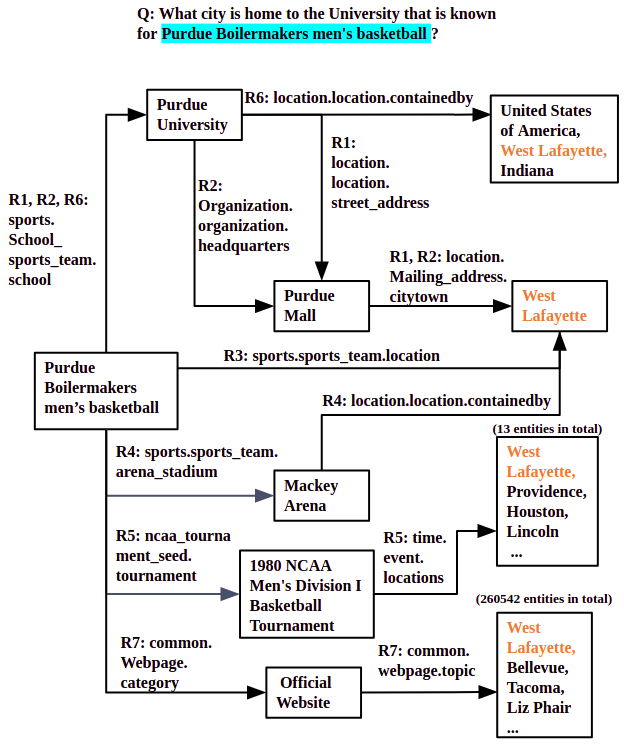
\includegraphics[width=1\linewidth]{figs/fig1.png}
 \caption{One QA example with Multiple Relation Paths from \textsc{ComplexWebQuestion}-1.1. The blue color highlighted is the extracted topic entity. Each square represents an entity, and the arrows represent the relations. Relation path $R_1$ to $R_4$ are the good ones containing meaningful relation paths to the final answer. $R_5$ and $R_6$ are the worse paths that generate a larger final answer set containing some wrong entities. $R_7$ is the worst one as its relation path is totally not interpretable and the answer set is huge.}
 \label{QAPaths}
\end{figure}

\section{Introduction}

Knowledge-based question answering (KBQA) is the task of finding answers to questions by processing a structured knowledge base $\mathcal{KB}$. %where the beliefs are stored as triples containing two entities and the relation linking them. 
A $\mathcal{KB}$ consists of a set of entities $\mathcal{E}$, a set of relations $\mathcal{R}$, and a set of literals $\mathcal{S}$ \cheng{and as set of facts?}. A knowledge base fact is defined as $(h,r,t)$, where $h\in \mathcal{E}$ is the head entity, $t \in \mathcal{E} \bigcup \mathcal{S}$ is the tail entity/literal \cheng{when do we use literals?}, and $r\in \mathcal{R}$ is the directed relation between $h$ and $t$. To answer a simple single-relation question (\emph{i.e.} a 1-hop question) such as: ``Who is the president of the United States?'', %a KBQA system first identifies the topic/focus entity (\emph{i.e.} United States) and the relation (\emph{i.e.} ``president '') asked in the question, then searches for the entity by matching the entity-relation tuple $\textless$United States, president, $?\textgreater$ over KB. \kalpa{use of a topic entity is approach specific. Many KBQA systems exist that do not use topic entity. E.g., template based QA}
a typical KBQA system first identifies the entity (\emph{i.e.} United States) and the relation (\emph{i.e.} ``president'') asked in the question, and then searches for the answer entity by matching the entity-relation tuple $\textless$United States, president, $?\textgreater$ over $\mathcal{KB}$.


While the single-hop question can be answered by searching a predicate relation in $\mathcal{KB}$, it is much harder to answer more complex multi-hop questions containing multiple entities and relations with constraints. For instance, for complex compositional questions, it is not easy to extract all the correct relations together withhead and tail entities in the right order. For complex conjunction questions \cheng{need to explain what conjunction question means}, it is often difficult to extract all the reasoning paths involved, and combine their results in the end. 

Most prior work on multi-hop KBQA focuses on learning the single given ground truth relation path for each question, and outputting  the most possible reasoning path during prediction \cheng{we need to unify "reasoning path" and "relation path"}. In reality, however, it is often the case that there exist many alternative relation paths that all lead to the correct answer, and these are not provided as ground truth by the human annotators. %It is hard to pre-define the maximum number of hops in a complex question because different questions may need different number of hops to reach their answers.
%\kechen{list a few problems (1) it hard to control number of hops. (2) how to decompose a complex question into sub-question. (3) ...} 
%\kechen{add something to explain why the above two points lead to decomposing into two sub-tasks?}
 %with random walks \cite{DBLP:conf/emnlp/GardnerTKM13} or is formulated as a Markov decision process (MDP) based reinforcement learning problem~\cite{DBLP:conf/emnlp/XiongHW17}.
%\kechen{Most of the existing KBQA systems cannot handle these two issues simultaneously. People have to pre-define different rules to solve different type of complex querys. For example, list a few work using different pre-defined strategy to solve complex QA.}%1. use different model to train, 2. neural program
%traditional approaches consider all the paths and search for the best path among them, where their searching algorithms either leverage path-ranking algorithms with random walks \cite{DBLP:conf/emnlp/GardnerTKM13} or is formulated as a Markov decision process (MDP) based reinforcement learning problem~\cite{DBLP:conf/emnlp/XiongHW17}. Since the complexity of the searching process can grow exponentially when the number of hops increase, some recent researches add decision markers or a terminal relation to decide whether a searching path should terminate or continue, in order to reduce the searching space and complexity \cite{DBLP:conf/naacl/ChenCCNK19}.
%It is commonly observed that, by using the above mentioned algorithms, the extracted relation path may not always be the best one or even can be a wrong one. The main reason is because during training, for one question, their models are trying to learn and fit to only one possible relation path, which is given as its ground truth. \kechen{while during prediction only predict one path}In reality, however, it is always possible that there exists many other relation paths leading to the answer, which are not given as ground truth. 
For example, Figure \ref{QAPaths} shows 7 relation paths $R_n={e^n_0\rightarrow r^n_1 \rightarrow e^n_1 \rightarrow \cdots \rightarrow e^n_{ans}}\ (n=\lbrace 1, \dots, 7 \rbrace)$ leading to the correct answer entity ``West Lafayette'' for the question \textit{``What city is home to the University that is known for Purdue Boilermakers men's basketball?''} %\footnote{An exchangeable way to define relation path is omitting entities in the definition, because entity is determined by given the topic entity, relations, and the knowledge base. For simplicity, we simplify this relation path definition as a list of sequential relations $(r_{1}^n, r_{2}^n, \cdots, r_{T}^n)$ in the following part of this paper.}
, but only the relation path R1 is labeled as the ground truth relation path in the dataset. \cheng{These statements are too general and speculative. Better to explain with concrete failure cases.} \fix{It is unlikely for the model to infer all possible relation paths that can direct the model to the answer set containing the final answer, only based on one given training path. It is not even possible for the model to differentiate the good paths from the bad ones, which are some unreasonable paths also leading to the answer sets %containing our target answer
or some reasonable paths leading to a large predicted set which contains both correct answer and noisy results.} \cheng{We need to first explain what we mean by good paths, which are good paths, and then claim that existing methods cannot disinguish good ones from bad ones} As the example given in Figure \ref{QAPaths}, relation paths $R_1$ to $R_4$ are the good ones containing meaningful relation paths to the final answer, by executing different number of hops. \cheng{We cannot simply define good paths as "meaningful" paths. This is not a useful definition. Define a good path as a path that leads to a small answer set?} Comparatively, relation paths $R_5$ and $R_6$ lead to a larger final answer set containing not only the correct answer entity but also many other wrong entities. These paths can be treated as inferior to the top 4 paths, since they give some extra invalid answers besides the correct one. \cheng{It is not clear where the discussion on good path vs bad path comes from. Why do I need to care about good path vs bad path? Who set this standard for good path? Is that us, or is that implied by the f1 evaluation metric? Is that for better interpretability?} In the example, path $R_7$ is even worse as its relation path is totally not interpretable plus the final answer set is exaggeratedly large which mainly contains invalid answers, hence should not be considered as a positive relation path training sample for this question. \cheng{Here we need a summary of why existing methods are bad}

%Although someone may claim that we can use multiple relation paths as ground truths for one question to improve the coverage and performance, it is still not feasible to label all valid relation paths considering the complexity of ground truth label preparation. 
%\kechen{combine this paragraph with the next paragraph? now we have two separate paragraphs to first introduce the issue and then use an example to explain it. should we combine them together?}

In this paper, we propose an end-to-end multi-hop KBQA system, which can leverage the training information from multiple relation paths, and learn the good relation paths over the inferior or the bad ones, based on only one given relation path annotation per instance (as in most KBQA datasets) or even no relation path annotation. We model the relation path as a latent variable, and propose supporting training and prediction methods. Experimental results show that the system can output diverse relation paths, and reward the ``better'' paths over the inferior ones by assigning ``better'' paths higher probabilities. Our method can be applied to most KBQA systems to predict entity and relation, and can be used with any model architecture. We achieve strong performance on three popular KBQA datasets for single-hop and multi-hop questions. \kechen{Especially, we show that our model perform extremely well on difficult dataset vs. simple dataset, multi-hop question vs. single question, and multiple path question vs. single path question.} %taking the size of their answer set into consideration, \emph{i.e.} the larger is the final answer set, the worse is a relation path, as it contains more irrelevant answer information. \kechen{modify the last sentence} %We also use a sampling approach to filter the wrong paths like $R_8$ in our example. 
% Specifically, we make the following contributions:\\
% 1. We introduce a novel multi-hop KBQA structure, which can predict the relation sequence of any length without pre-defining the number of maximum hops and generate final answers at the last hop.\\
% 2. We design a novel loss function using latent variables, such that the system can be trained without being given any ground truth relation path, or by leveraging more valid training paths information even if one ground truth path is given. We also give detailed analysis to demonstrate the benefits of using the new loss function.\\
% 3. We achieve state-of-the-art performance on three popular KBQA dataset containing single-hop and multi-hop questions.
%Specifically, we make the following contributions:
%\begin{enumerate}
%    \item We introduce a novel multi-hop KBQA system, which can leverage the information from multiple relation paths. %predict the relation sequence of any length without pre-defining the number of maximum hops and generate final answers at the last hop.
%    \item We design a novel loss function and the corresponding training and prediction methods. Detailed analysis is given to demonstrate the benefits of using this new loss function.
%    \item We achieve state-of-the-art performance on three popular KBQA datasets for single-hop and multi-hop questions.
%\end{enumerate}
